%!TEX root = ../report.tex


\chapter{Design}\label{ch:design}
%TODO @maurits image is not inserted at correct location and citation text is only possible above of figure, couldnt figure out a way around that
\subsection{Design artefacts}
This part of the document will present the artefacts which have been developed during the design phase.

\begin{figure}[h]
	\centering
	\caption{Service interaction concept designed for admin panel}
	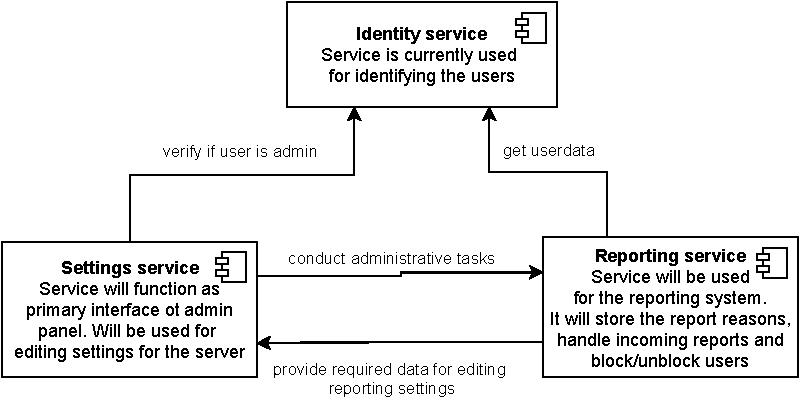
\includegraphics[width=1.0\textwidth]{./images/component_interaction.pdf}
	\label{fig:componentInteraction}
\end{figure}

Figure~\ref{fig:componentInteraction} shows a concept for the components that will have to be added for the admin panel. The Settings service will function as the rest interface to the Admin panel. To this point it will interact with the identity service for verifying if the settings are actually being changed by an administrator user. It will also work with the reporting service, which is also another new service in charge of handling the reporting system, to conduct administrative tasks like changing the reasons people can be reported for. 

\begin{figure}[h]
	\centering
	\caption{Service interaction concept designed for admin panel}
	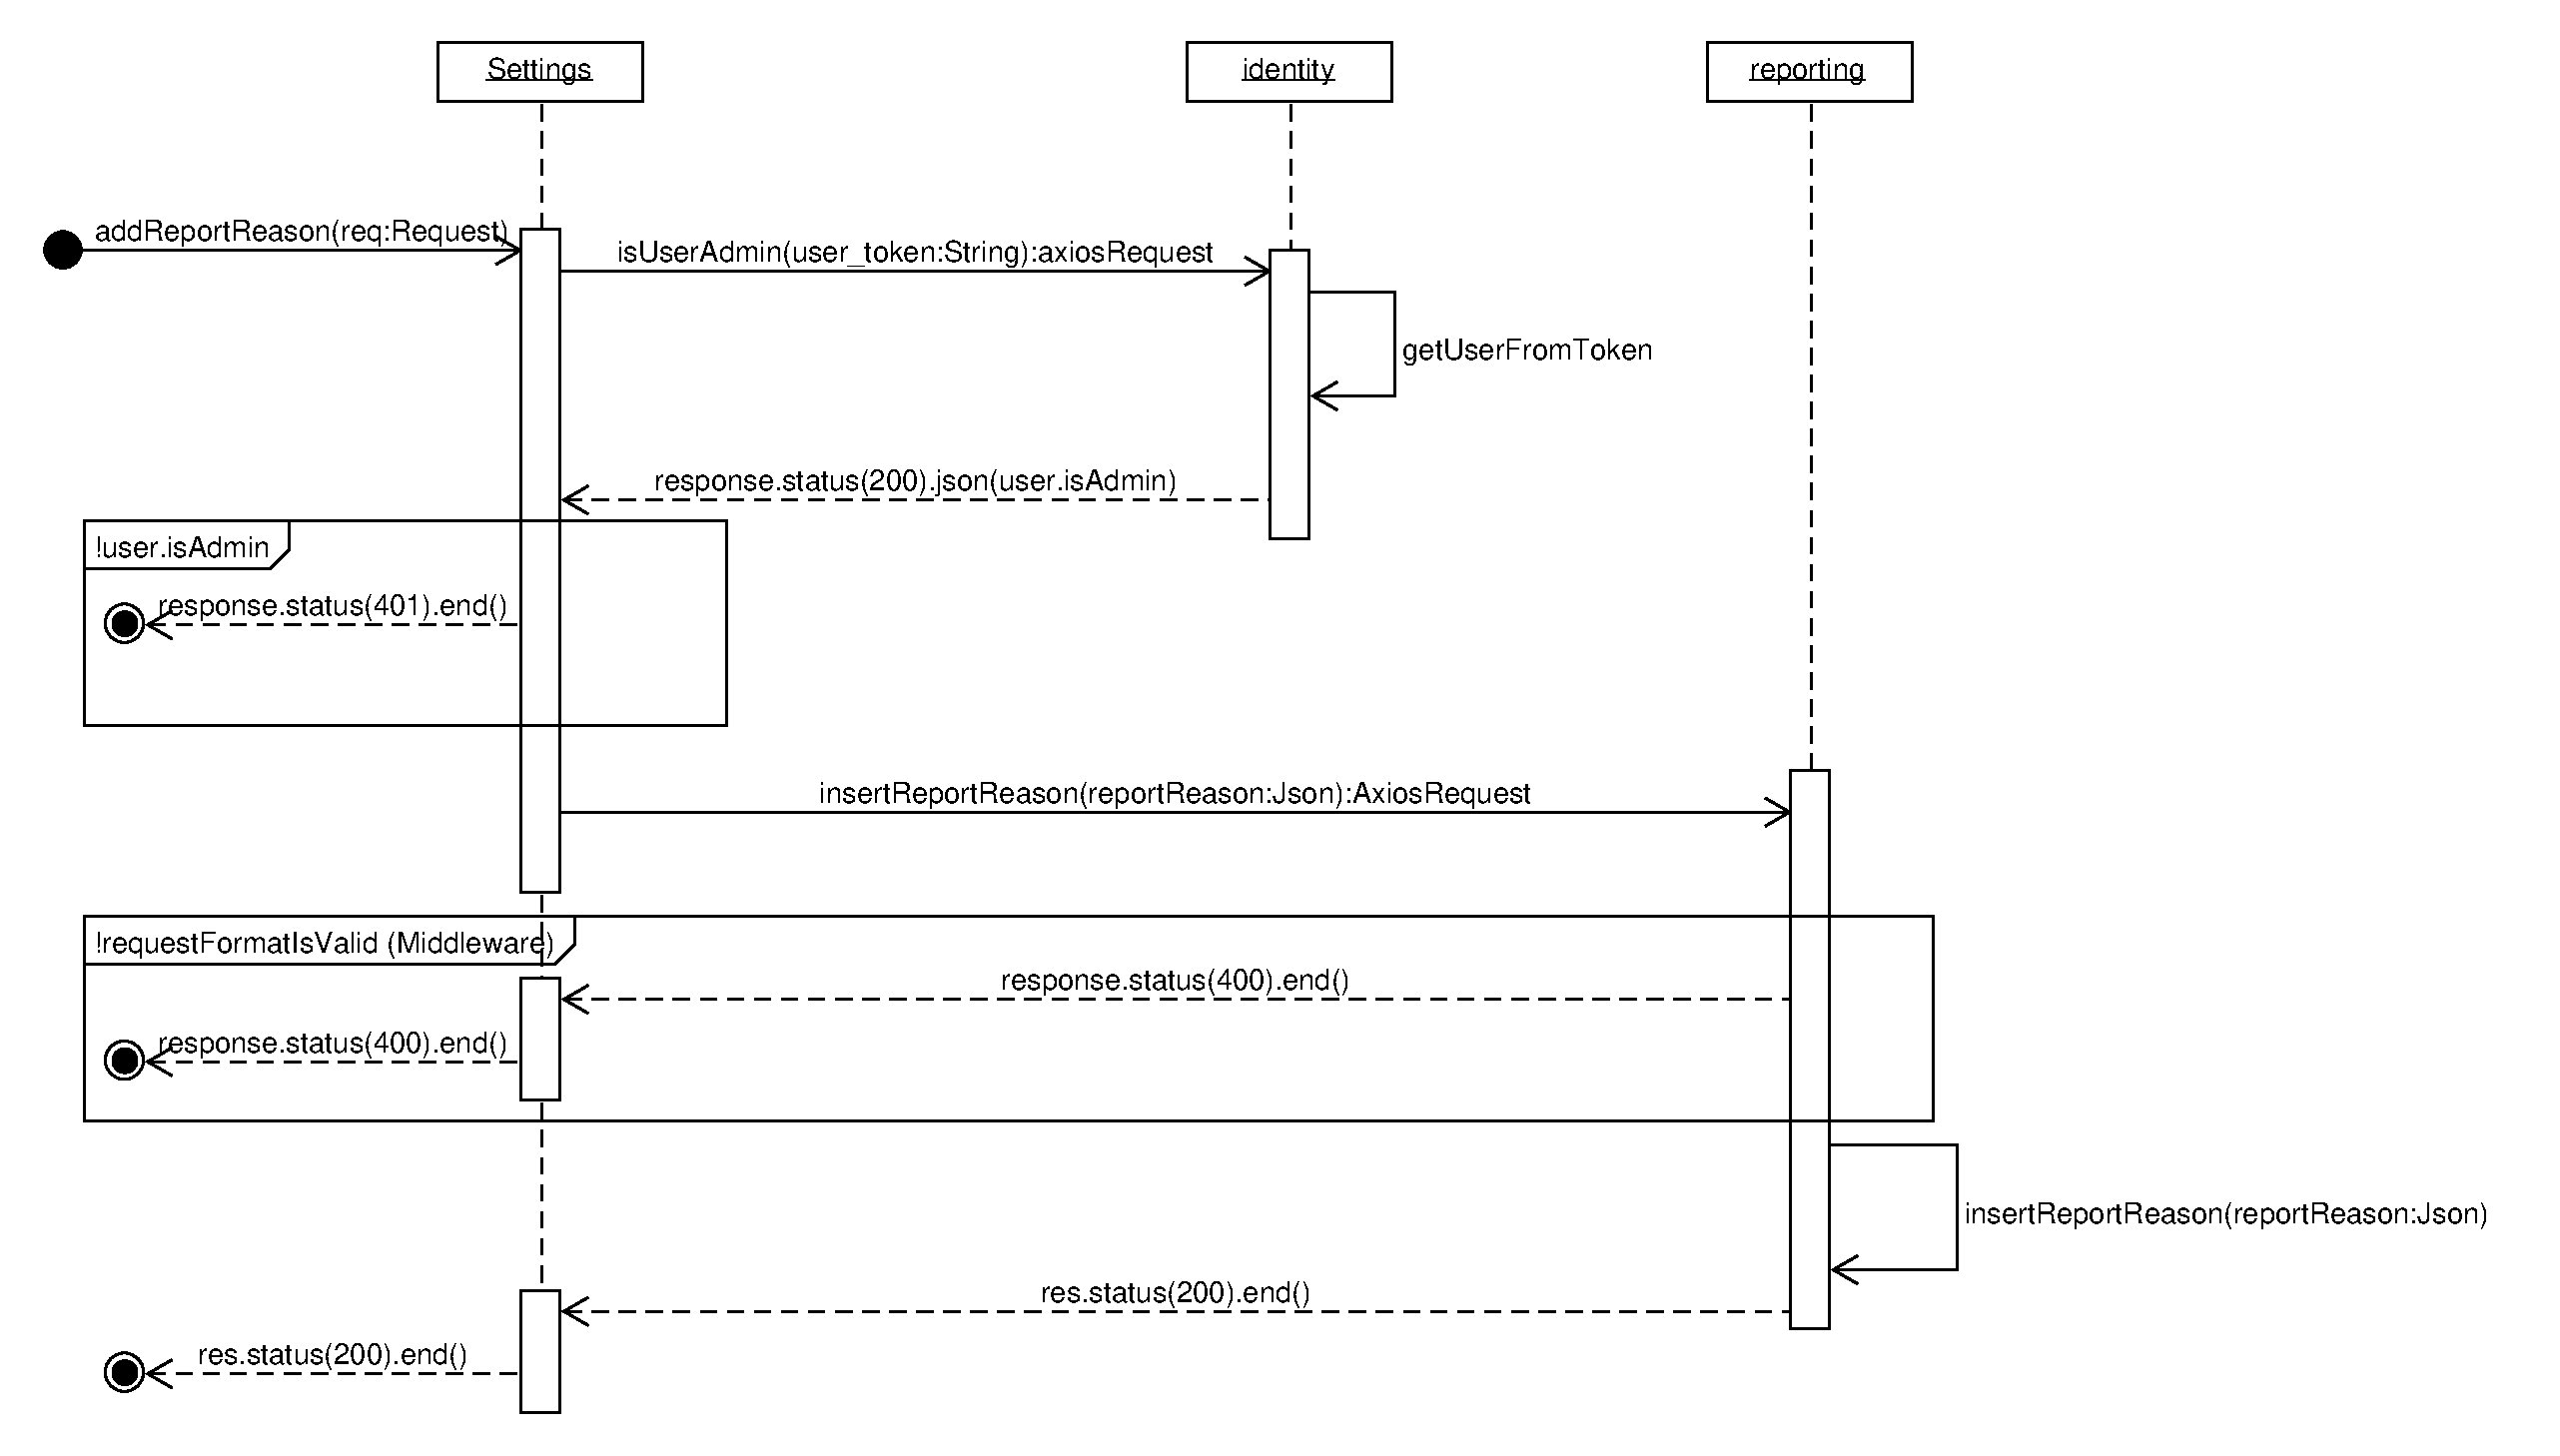
\includegraphics[width=1.0\textwidth]{./images/SequenceDiagram_AddReportReason.pdf}
	\label{fig:sequenceDiagramAddReportReason}
\end{figure}

Figure~\ref{fig:sequenceDiagramAddReportReason} shows the sequence diagram for conducting the administrative task of adding a report reason. This diagram has been created in order to further visualize the responsibility and interaction between the existing identity service and the two new services (settings and reporting)

\section{Network Design}\label{sec:network-design}

\subsection{Application Layers}\label{subsec:application-layers}
% TODO @joernneumeyer & @mauritsvanderzee

\subsection{Network Architecture}\label{subsec:network-architecture}
% TODO @joernneumeyer & @mauritsvanderzee
% Umlet diagrams ..?

\subsection{Port distribution}\label{subsec:port-distribution}

% TODO @all add descrptions to table
\begin{table}[]
    \begin{tabular}{lll}
        \textbf{Port} & \textbf{Service}                               & \textbf{Description} \\
        8086          & Default Application Port                       & TODO @all            \\
        3000          & Identity Service                               & TODO @all            \\
        3001          & Chat service over HTTP                         & TODO @all            \\
        3002          & Chat service over SocialStuff/Trale connection & TODO @all
    \end{tabular}\label{tab:table}
\end{table}

\subsection{Database management system}\label{subsec:database-management-system}
% TODO @all Which dbms, why, schemas, which tables columns constraints etc.

\lipsum[2-4]
